Data used for this project:
\subsection{Datasets}
    \subsubsection{ \label{secondModel} Face Mask Detection Dataset \cite{face-mask-detection}}
        Comprised of the following three classes:
        \begin{itemize}
            \item Face with mask
            \item Face without mask
            \item Mask worn incorrectly
        \end{itemize}

        Classes Distribution: (Equal number of images per class, to eliminate bias)
        \begin{itemize}
            \item mask\_weared\_incorrect: 2997
            \item with\_mask: 2997
            \item without\_mask: 2997
        \end{itemize}


    \subsubsection{\label{firstModel} Face Mask Dataset \cite{face-mask-detection} \&  Natural Images Dataset \cite{natural-images}}
        A custom superset of both \cite{face-mask-detection} \&  \cite{natural-images}, Comprised of the following classes:
        \begin{itemize}
            \item airplane
            \item car
            \item cat
            \item dog
            \item flower
            \item fruit
            \item mask\_weared\_incorrect
            \item motorbike
            \item with\_mask
            \item without\_mask
        \end{itemize}

        Classes Distribution:
        \begin{itemize}
            \item airplane: 727
            \item car: 968
            \item cat: 885
            \item dog: 702
            \item flower: 843
            \item fruit: 1000
            \item mask\_weared\_incorrect: 2997 --> 1000
            \item motorbike: 788
            \item with\_mask: 2997 --> 1000
            \item without\_mask: 2997 --> 1000
        \end{itemize}

\subsection{Transformations used for data}
\begin{itemize}
    \item Random Horizontal Flip: Horizontally flip the given image randomly with a given probability
    \item Random Resized Crop: Crop the given image to random size and aspect ratio
\end{itemize}


\begin{figure}[H]
    \centering
    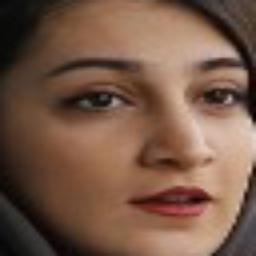
\includegraphics[width=0.3\textwidth]{Person1.jpg}
    \caption{Cropping Sample}
    \label{fig:First}
\end{figure}
